\chapter{System Development}
In order to achieve the goal of this project, the workflow and whole system architecture was carefully planned from the very beginning. To achieve high quality results, every part of the system had to produce satisfactory artifacts. Therefore, the system is made of independent parts, all of which have been separately implemented, tweaked and evaluated. Furthermore, as first story and risk emergence detection in financial domain had not been widely researched yet, there has been a lot of experimentation involved.

The goal of this project was to identify the emerging risks. Therefore, firstly the known, constant risks were filtered out (sentences representing them). Then, the remaining sentences were grouped and processed in a way that extracts the emerging risks.

\section{Requirements}
\begin{enumerate}
\item Acquire and organise the large dataset and its metadata.
\item Remove all non-textual data from the documents.
\item Isolate and extract risk factor sections from reports.
\item Perform any optional data cleaning processes.
\item Analyse the dataset using word and n-gram term frequencies and TF-IDF.
\item Classify sentences into one of constant known risks or keep it in remaining emerging risk class.
\item Group remaining risk class sentences by their similarity and/or report release year.
\item Apply LDA model on different groupings in order to extract topics.
\item Analyse the final results.
\end{enumerate}

\section{System Architecture}
\begin{figure}[H]
\begin{center}
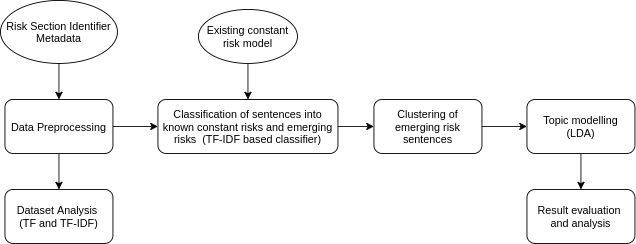
\includegraphics[scale=0.6]{projectArchitecture.png}
\label{fig:architecture}
\caption{System Architecture Diagram}
\end{center}
\end{figure}

This system architecture diagram provides a high-level overview of the system design for this project. Every part of the pipeline, while not fully decoupled is mostly independent and takes in the output of the previous part, as well as some additional data if needed (ellipse parts).

Such architecture provides a capability to tweak, evaluate and reimplement different parts of the pipeline independently as long as the output follows the same format and logic. This is a crucial feature for such project, as major improvements can be made iteratively after gathering and evaluating the end results.

The system was implemented using Python and some common python libraries such as nltk \cite{nltkhome}, scikit-learn \cite{sklearnhome} and others.

\section{Data Preprocessing}
Preparing the dataset is important to achieve high-quality results. While it may seem as a trivial and easy task it proved to be fairly complex, because of inconsistent layout, HTML, structure of reports and the size of the dataset. Therefore, data preprocessing has been divided into three main tasks:
\begin{itemize}
\item parsing the documents into text
\item extracting risk factor sections
\item data cleaning, normalisation
\end{itemize}

\subsection{Document Parsing}
The first step in data preprocessing pipeline was parsing HTML and removing any non-textual elements, keeping only the textual information from the document. This was achieved by using lxml library's HTML parser in Python \cite{lxmlhtml}.

The initial parsing was long and challenging task, which required special handling, because the dataset size was over 600GB. Parsing has reduced the dataset size from $\sim$600GB to $\sim$76GB, which made work with dataset more feasible.

\subsection{Risk Section Extraction}
As this project is focused on working with risks, it was decided to focus only on risk section in the document, which is most often called "Item 1A. Risk Factors". However it is not always clearly and consistently titled section. Fortunately, Dr. Stefan Petry has provided some metadata which includes identifiers of section start and section end sentences. This data came in handy, but it was still not enough in some cases, therefore some additional processing was done in order to standardize whitespaces and capital letters. Furthermore, as often there were more than one matches of those start and end sentences, some additional algorithmic logic was added.

The simple algorithm first finds every start and end sentence occurence and then it chooses such combination, that it is the longest text extract, not having any start or end sentence occurences in it. This way, it was ensured that detected sentences were in fact referring to the section start and end rather than table of content entries or references from other parts of the document.

Furthermore, to filter out outliar risk sections and various risk extraction errors, only the extracts over 1,000 characters and those that were shorter than one-third of the respective report were used. The optimal outliar filtering parameters have been derived by sampling the outliars as well taking into account how many potential risk sections get discarded.

The quality of extraction was verified primarily by random manual sampling, of various length and parameter risk section extracts. However, some additional features were covered by automatic testing of all risk section extracts. One of such features, was checking how many risk section extracts ended with a phrase "unresolved staff comments" as it was fairly common and easily testable parameter, and 35,714 of extracts had that phrase in the end which was a strong suggestion to the correct ending of the extract.

The resulting dataset consisted of 43,795 (out of 53,093 reports) risk sections, amounting to $\sim$2.1GB of data.

\subsection{Normalisation}
Most often for applications dealing with text there are a lot of text normalisation done before. Common examples include case folding, lemmatization and stemming. In this project it was decided that most of those techniques should not be used as a default for all the data due to some of the pipeline steps requiring standard word forms. Therefore, the only normalisation technique applied at data preprocessing step was stopword removal (removing common words with little meaning i.e. and, or, but), stopwords were only left and used at the dataset profiling step.

In some parts of the pipeline further normalisation techniques were used or experimented with (mainly stemming). Also to remove punctuation, word tokenisation was used and punctuation signs were not taken into account in any steps except for dataset profiling.

\section{Dataset Profiling}
Dataset analysis can play an important role at the start of the project, as it provides a better understanding about the project's context. Therefore, in this project term frequency and TF-IDF has been used on words and n-grams to gain some insight into important features of the risk sections.

\subsection{TF}
Term frequency analysis while does not necessarily provide too much insight it can still give some ideas about most common words in the dataset. 

This analysis has been performed on the whole risk section dataset, including stopwords (which can be ignored when analysing). The analysis was run on words with and without using stemming as well as on bi-grams and tri-grams without using stemming. Counting was implemented using Python's Counter while word tokenisation, stemming and n-gram generation was implemented by nltk library \cite{nltkhome}.

\begin{table}[H]
\centering
\begin{tabular}{|l|c|}
\hline
Word & Count \\
\hline
may & 384,301\\\hline
could & 329,270\\\hline
busi & 244,587\\\hline
financi & 214,073\\\hline
result & 287,312\\\hline
risk & 134,397\\\hline
regul & 96,869\\\hline
cyber & 2,031\\\hline
agricultur & 2,017\\\hline
aviat & 1,088\\\hline
\end{tabular}
\caption{Random Stemmed Word Term Frequency Extract}
\label{table:tfstem}
\end{table}

\begin{table}[H]
\centering
\begin{tabular}{|l|c|}
\hline
N-gram & Count \\
\hline
results of operations & 81,660\\\hline
financial condition & 71,326\\\hline
adversely affect & 67,969\\\hline
material adverse effect & 36,237\\\hline
december 31 & 26,049\\\hline
rules and regulations & 2,617\\\hline
cyber attacks & 522\\\hline
\end{tabular}
\caption{Random (2,3)-gram Term Frequency Extract}
\label{table:tfngrams}
\end{table}

The data extracts can provide a few important insights:
\begin{itemize}
\item A lot of speculative, future oriented language ('may', 'could', 'would')
\item A lot of common business performances terms ('result', 'financial')
\item Negatvie sentiment can be found ('adeversely affect', 'risk')
\item Constant risks can be found ('financi', 'regul', 'rules and regulations')
\item Newly, less popular risks can be found when looking at less frequent terms ('cyber', 'cyber attacks', 'aviat', 'agricult')
\item Importance of 31st December, end of the year in the context of the reports.
\end{itemize} 

\subsection{TF-IDF}
Term frequency - inverse document frequency analysis is another useful early stage analysis tool. While usually TF-IDF would be used on document basis, calculating it on whole dataset, it can provide insights into important keywords in the dataset, potentially, uncovering some early clues about the risks that can be found in the dataset.

Because usually TF-IDF would be calculated on document basis, most libraries are implementing it that way, therefore a custom implementation of TF-IDF was built. Using TFIDFVectorizer from scikit-learn package \cite{sklearnhome} inverse document frequencies were extracted, then all that was left to do was combined inverse document frequencies with previously calculated term frequencies (term frequencies of the whole dataset).

This custom TF-IDF calculation was run on the same dataset and its preprocessing variants as term frequency analysis (stemmed word, non-stemmed words, bi-grams, tri-grams).

\begin{table}[H]
\centering
\begin{tabular}{|l|c|}
\hline
Term & TF-IDF \\
\hline
loans & 34701.2115769626\\\hline
nuclear & 27130.4207448989\\\hline
decommissioning & 16524.391082016\\\hline
intellectual property & 14121.7057905634\\\hline
oil and gas & 13950.7980818019\\\hline
the merger & 11483.1921567622\\\hline
information technology & 7674.83078275194\\\hline
credit risk & 6943.80076762693\\\hline
information technology systems & 5413.98271394986\\\hline
cyber & 4166.54304462543\\\hline
cyber security & 1517.5070726361\\\hline
\end{tabular}
\caption{Random (1,2,3)-gram TF-IDF Extract}
\label{table:tfidfall}
\end{table}

Table \ref{table:tfidfall} illustrates some of the terms, which have relatively high TF-IDF scores (the scores span from $\sim$100,000 to $\sim$0.5). It can be seen that this method already extracts some potential risk mentions, such as \textit{loans, nuclear field specific risks, decomissioning} and others, as well as lowers the score of some constant common risks such as \textit{credit risk}. However, compared to those risks, emerging risks such as cyber securiy and information technology are still often ranked lower than a lot of constant risks.

\section{Classification of Sentences Into Constant and Emerging Risks}
\label{sec:classification}
During the design phase of the project, it was decided that to achieve insights into less common, newly emergin risks, there was a need to filter out the constant known risks first, leaving only the sentences with potential emerging risks.

\subsection{TF-IDF Based Classification Algorithm}
Due to having only keywords for topics available and not a full ontology, traditional sentence classification models were not feasible in this project as they are mostly trained on labeled sentences. The choices were to either use the provided topic keywords as seed words or to create a TF-IDF based classifier. As TF-IDF based method implementation was much simpler to implement it was a first choice. Furthermore, it was used in a similar context in research in which they used TF-IDF to vectorize sentences and base the classification on cosine similarities\cite{tfidfclassificationresearch}. However there was a major difference in the approach because they used labeled sentences as their training data, which was not feasible in this project.

The custom model was implemented by first generating the vector of the topic, which was done by adding all the keywords to one sentence and vectorizing it using TFIDFVectorizer from scikit-learn package in Python \cite{sklearnhome}. Then every sentence from the dataset, which is longer than 5 words is converted to TFIDF vector as well and for every sentence the nearest topic vector is found by calculating their cosine similarities. Then based on the threshold parameter and the similarity of the sentence to the most similar topic it is either classified as one of 30 constant risks or as a newly emerging risk sentence (unclassified class). After a lot of experimentation this parameter has been set to be 0.05 (meaning, that if similarity $<$0.05 then it is an unclassified emerging risk sentence).

\subsection{Evaluation of Classification}
The result of this classification yielded 11.01\% of all sentences to remain unclassified (i.e. potential emerging risk sentences). The testing of this classification method was based mainly on manual sampling of different similarity score sentences, from such evaluation the accuracy of classified class was extremely high ($\sim$90\%). The sentences that were left unclassified also seemed promising with $\sim$75\% of them having potential to identify emerging risks. However, the evaluation was very subjective as a lot of sentences were ambiguous.

{\renewcommand{\arraystretch}{2}%
\begin{table}[H]
\centering
\begin{tabular}{|S|c|c|}
\hline
Sentence (without stopwords) & Topic label & Similarity \\
\hline
Debt equity capital may continue available us favorable terms, all. & Financing Uncertainty & 0.170663803\\[5pt]\hline
inability obtain financing favorable terms could adversely affect results operations financial condition. & Financing Uncertainty & 0.271898346\\[5pt]\hline
addition, loan agreements contain financial covenants require us comply specified financial ratios tests relating fixed charge coverage minimum working capital tangible net worth levels. & Financial Liability & 0.101999065\\[5pt]\hline
Acquisitions expose us risks, including risk may unable effectively integrate acquisitions. & Real Estate & 0.071584165\\[5pt]\hline
\end{tabular}
\caption{Constant risk sentence examples and their similarity score to the most similar constant risk topic}
\label{table:classifiedclassexample}
\end{table}

From Table \ref{table:classifiedclassexample} it can be seen that categorized sentences are indeed corellating with constant financial risks, such as financing, loans and acquisitions.

\begin{table}[H]
\centering
\begin{tabular}{|Mc|}
\hline
Sentence (without stopwords) &\\
\hline
FAA, airlines others industry heightened sensitivity scrutiny respect compliance approved maintenance procedures.&\\[5pt]\hline
recently, demand air transportation United States abroad decreased due adverse changes deterioration U.S. global economies.&\\[5pt]\hline
example, European Union (EU) China two among growing number jurisdictions enacted recent years restrictions use lead, among chemicals, electronic products countries considering similar restrictions.&\\[5pt]\hline
past year, cyber-attacks become prevalent much harder detect defend against.&\\[5pt]\hline
\end{tabular}
\caption{Uncategorized, potential risk sentences}
\label{table:uncategorizedclassexample}
\end{table}

Table \ref{table:uncategorizedclassexample} shows some of the examples of potential emerging risk sentences, which refer to specific events in the airline industry, specific restrictions to electronic products and finally cyber attacks.

\section{Clustering Emerging Risk Sentences}
Even after filtering out constant risk sentences, there were still many sentences left that were repeated in the same documents year after year. Therefore, it was decided to try to organise them by similarity and this way have the first unique occurence of the sentence and therefore the first occurences of potential risks.

\subsection{Word Embedding Representation}
\label{sec:wordembeddingsentenceuse}
For word and sentence representation, word embeddings were chosen as they are a good modern and fairly universal technique used for text processing tasks. Furthermore, they can be pre-trained on the dataset to work in the specific context and that has been previously done on this specific dataset. 

The pre-trained financial word embedding model \cite{10kwordembeddings} was imported, then every sentence was converted into a bag-of-words, then every word was using the word embeddings translated to vector and these from these vectors the mean average was calculated which was the representation of the sentence.

\subsection{K-Means Clustering}
First consideration was using one of the most standard clustering algorithms, K-Means clustering. However there was a major drawback with it as it had to have pre-set number of clusters. That meant that there was no good way to cluster sentences into clusters with assured first occurences.

However, it was still tried out in an attempt to use it as a topic modelling tool, which would represent the topic by its center. However that attempt failed, because most of the cluster centres were not represented by sentences and the results were impossible to convert back to textual form.

One other limitation discovered in various experimentations with K-means was that it is using Euclidean distance and changing this into cosine distance instead requires converting k-means algorithm into spherical k-means.

\subsection{Density-Based Spatial Clustering of Applications with Noise (DBSCAN)}
\label{sec:dbscanclusters}
DBSCAN is much less common clustering algorithm. However it has a very important advantage of not needing to set the number of clusters, but providing the maximum distance ($\varepsilon$) to put data points into cluster instead and minimum size of the cluster. Such behaviour makes it perfect for clustering sentences into clusters of similar meaning and finding the first mentions. Furthermore, its implementation enables an easy choice of distance metric. Therefore cosine distances can be easily used instead of Euclidean distance. Finally, it also filters out the "noise", which in this case are the sentences that do not reappear in a similar form in documents.

The DBSCAN in this projected was implemented using scikit-learn package \cite{sklearnhome} and passing the sentence vectors created from word embeddings (as described in Section \ref{sec:wordembeddingsentenceuse}). The $\varepsilon$ through experimentation was chosen to be 0.1 and minimum cluster size was chosen to be 2. The clustering algorithm processed 1,191,452 potentially emerging risk topic sentences, 142,897 of which were considered to be "noise"(not reoccuring) and the rest were clustered into 156,930 clusters.

\begin{table}[H]
\centering
\begin{tabular}{|Mc|}
\hline
Sentence (without stopwords) &\\
\hline
Many files digitized employees working almost paperless environments.&\\[5pt]\hline
Many Company's files digitized employees working almost paperless remote environments.&\\[5pt]\hline
Many files digitized employees working almost paperless environments.&\\[5pt]\hline
Many Company's files digitized employees working almost paperless remote environments.&\\[5pt]\hline
Many files digitized employees working almost paperless environments.&\\[5pt]\hline
\end{tabular}
\caption{Single DBSCAN Cluster Example}
\label{table:dbscanclusterexample}
\end{table}

Table \ref{table:dbscanclusterexample} illustrates the similarity level among the sentences clustered into the same cluster. This example correlates with most clusters, in which the sentences are very similar among themselves. Therefore they can be treated as first occurence of particular sentence identifying clusters.

\section{Topic Modelling Using LDA}
Topic modelling was the final step of this project. It is also the part at which the final results can be seen. The topic modelling itself in this project is implemented by using LDA from scikit-learn package \cite{sklearnhome}. However, as there has been a lot of previous steps to prepare the data for topic modelling and only appply it on the part of the dataset that has a potential to contain emerging topics, the topic modelling is applied in three different experiments on the data prepared by previous steps.

\subsection*{Applying LDA on All Potentially Emerging Risk Sentences}
This is the most straightforward approach in which some insights can be gained and possibly new emerging risks identified. As it is fairly big document set, the topic number experimented with was between 30 and 50.

\subsection*{Applying LDA on The First Mentions of Similar Sentences}
By applying LDA only to the first mentions of the potential risk there can be uncovered most important newly emerging risks, which are mentioned in different ways and probably in different documents. Therefore such approach could potentially yield the most diverse set of newly emerging risks. The first mentions of reoccuring sentences were derived from DBSCAN clusters (described in Section \ref{sec:dbscanclusters}) and the year that the sentences were used in (from metadata). Then the LDA was applied on those sentences, by treating every sentence as a separate document. For this approach the number of topics experimented with was between 30 and 50 as well.

\subsection*{Applying LDA Separately For Every Year}
Applying LDA on a subset of data by dividing documents by year can reveal more about the topic distributions every year as well as it can directly show the risk changes throughout time. For this approach, after a lot of experimentation, the number of topics was chosen to be 10 for every year.

